\documentclass[aspectratio=169]{beamer}

\usepackage[spanish]{babel}
\usepackage[utf8]{inputenc}
\usepackage[T1]{fontenc}
\usepackage{lmodern}
\usepackage{graphicx}
\usepackage{booktabs}
\usepackage{amsmath}
\usepackage{array}
\usepackage{xcolor}
\usepackage{tikz}
\usepackage{pgfplots}
\pgfplotsset{compat=1.18}

\usetheme{Madrid}
\usecolortheme{default}
\setbeamertemplate{navigation symbols}{}
\setbeamertemplate{footline}[frame number]
\setbeamertemplate{itemize item}{\color{black}$\blacktriangleright$}
\setbeamertemplate{itemize subitem}{\color{black}$\bullet$}

\definecolor{ucmred}{RGB}{140,21,21}
\definecolor{softgray}{RGB}{82,82,82}
\setbeamercolor{title}{fg=ucmred}
\setbeamercolor{frametitle}{fg=ucmred}
\setbeamercolor{structure}{fg=ucmred}
\setbeamercolor{normal text}{fg=black,bg=white}

\graphicspath{{./}{figuras_memoria/}}

\title{Clasificaci\'on de artefactos arqueol\'ogicos}
\subtitle{Comparaci\'on entre modelos ligeros y transfer learning con EfficientNet}
\author{Mario Bermejo Cuervo \and Vanessa Stefani Carnero Olivares \\ Jes\'us Guti\'errez D\'iaz \and Aroa Ortiz Lominchar}
\institute{Universidad Complutense de Madrid\\Taller de tecnomatem\'atica}
\date{Abril de 2026}

\begin{document}

\begin{frame}
  \titlepage
  \begin{center}
    
\includegraphics[width=1.8cm]{logoUCM.png}
  \end{center}
\end{frame}

\begin{frame}{Problema y plan experimental}
\begin{columns}[T]
\column{0.58\textwidth}
\begin{itemize}
  \item Tarea: clasificar artefactos arqueol\'ogicos en 10 clases.
  \item Dataset: \texttt{cssl\_dataset}.
  \item Modalidades: \texttt{photos} y \texttt{drawings}.
  \item Dos bloques de comparaci\'on:
  \begin{itemize}
    \item modelos ligeros;
    \item transfer learning con \texttt{EfficientNet-B0}.
  \end{itemize}
\end{itemize}
\column{0.42\textwidth}
\small
\begin{block}{Bloque 1}
CNN\\
VAE + MLP\\
VAE + KAN
\end{block}
\begin{block}{Bloque 2}
EfficientNet + MLP\\
EfficientNet + KAN
\end{block}
\end{columns}
\end{frame}

\begin{frame}{Bloque 1: comparaci\'on entre modelos ligeros}
\begin{columns}[T]
\column{0.42\textwidth}
\small
\begin{tabular}{lcc}
\toprule
Modelo & Drawings & Photos \\
\midrule
CNN & 0.2250 & 0.2400 \\
MLP & 0.3500 & 0.2000 \\
KAN & 0.3417 & 0.1500 \\
\bottomrule
\end{tabular}

\vspace{0.5cm}
\begin{itemize}
  \item En dibujos, MLP y KAN superan a CNN.
  \item En fotograf\'ias, CNN es la m\'as estable.
  \item KAN queda cerca de MLP, pero no la supera.
\end{itemize}
\column{0.58\textwidth}
\centering
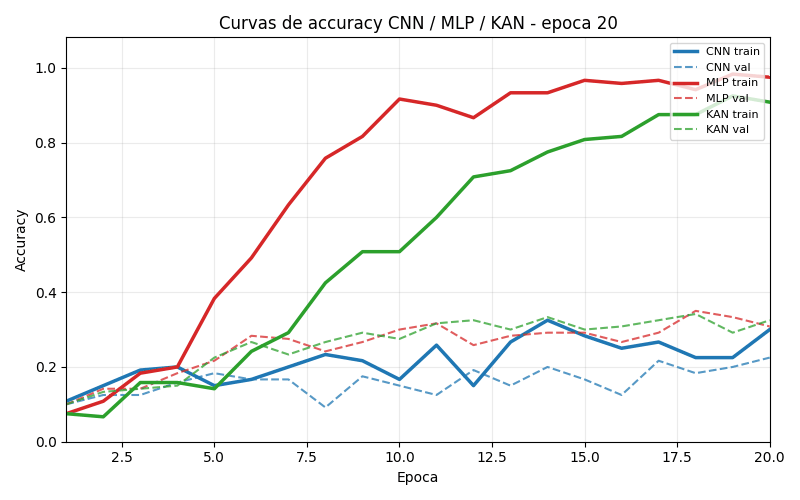
\includegraphics[width=\linewidth]{comparacion_accuracy_drawings_50-50_experiment_0.png}
\end{columns}
\end{frame}

\begin{frame}{Lectura del bloque 1}
\Large
\begin{itemize}
  \item El resultado depende mucho de la representaci\'on y del tama\~no del conjunto de entrenamiento.
  \item Con modelos ligeros, KAN es competitiva, pero no muestra una ventaja consistente frente a MLP.
\end{itemize}
\end{frame}

\begin{frame}{Bloque 2: EfficientNet con pares foto + dibujo}
\begin{columns}[T]
\column{0.58\textwidth}
\begin{itemize}
  \item Backbone compartido: \texttt{EfficientNet-B0}.
  \item Cada muestra es un par foto+dibujo del mismo artefacto.
  \item Se fusionan dos embeddings:
  \begin{itemize}
    \item foto,
    \item dibujo,
    \item diferencia absoluta,
    \item producto elemento a elemento.
  \end{itemize}
\end{itemize}
\column{0.42\textwidth}
\small
\begin{block}{Comparaci\'on}
Mismo backbone\\
Mismo split\\
Misma fusi\'on\\
\\vspace{0.2cm}
Solo cambia la cabeza final:
\begin{itemize}
  \item MLP
  \item KAN
\end{itemize}
\end{block}
\end{columns}
\end{frame}

\begin{frame}{Bloque 2: resultados cuantitativos}
\begin{columns}[T]
\column{0.44\textwidth}
\small
\begin{tabular}{lcccc}
\toprule
Modelo & \`Epoca & Train & Val & Hybrid \\
\midrule
MLP & 17 & 0.7307 & 0.3941 & 0.3892 \\
KAN & 24 & 0.4908 & 0.4483 & 0.4483 \\
\bottomrule
\end{tabular}

\vspace{0.5cm}
\begin{itemize}
  \item KAN mejora a MLP en validaci\'on.
  \item Tambi\'en mejora la m\'etrica h\'ibrida.
  \item Menor train acc., mejor generalizaci\'on.
\end{itemize}
\column{0.56\textwidth}
\centering
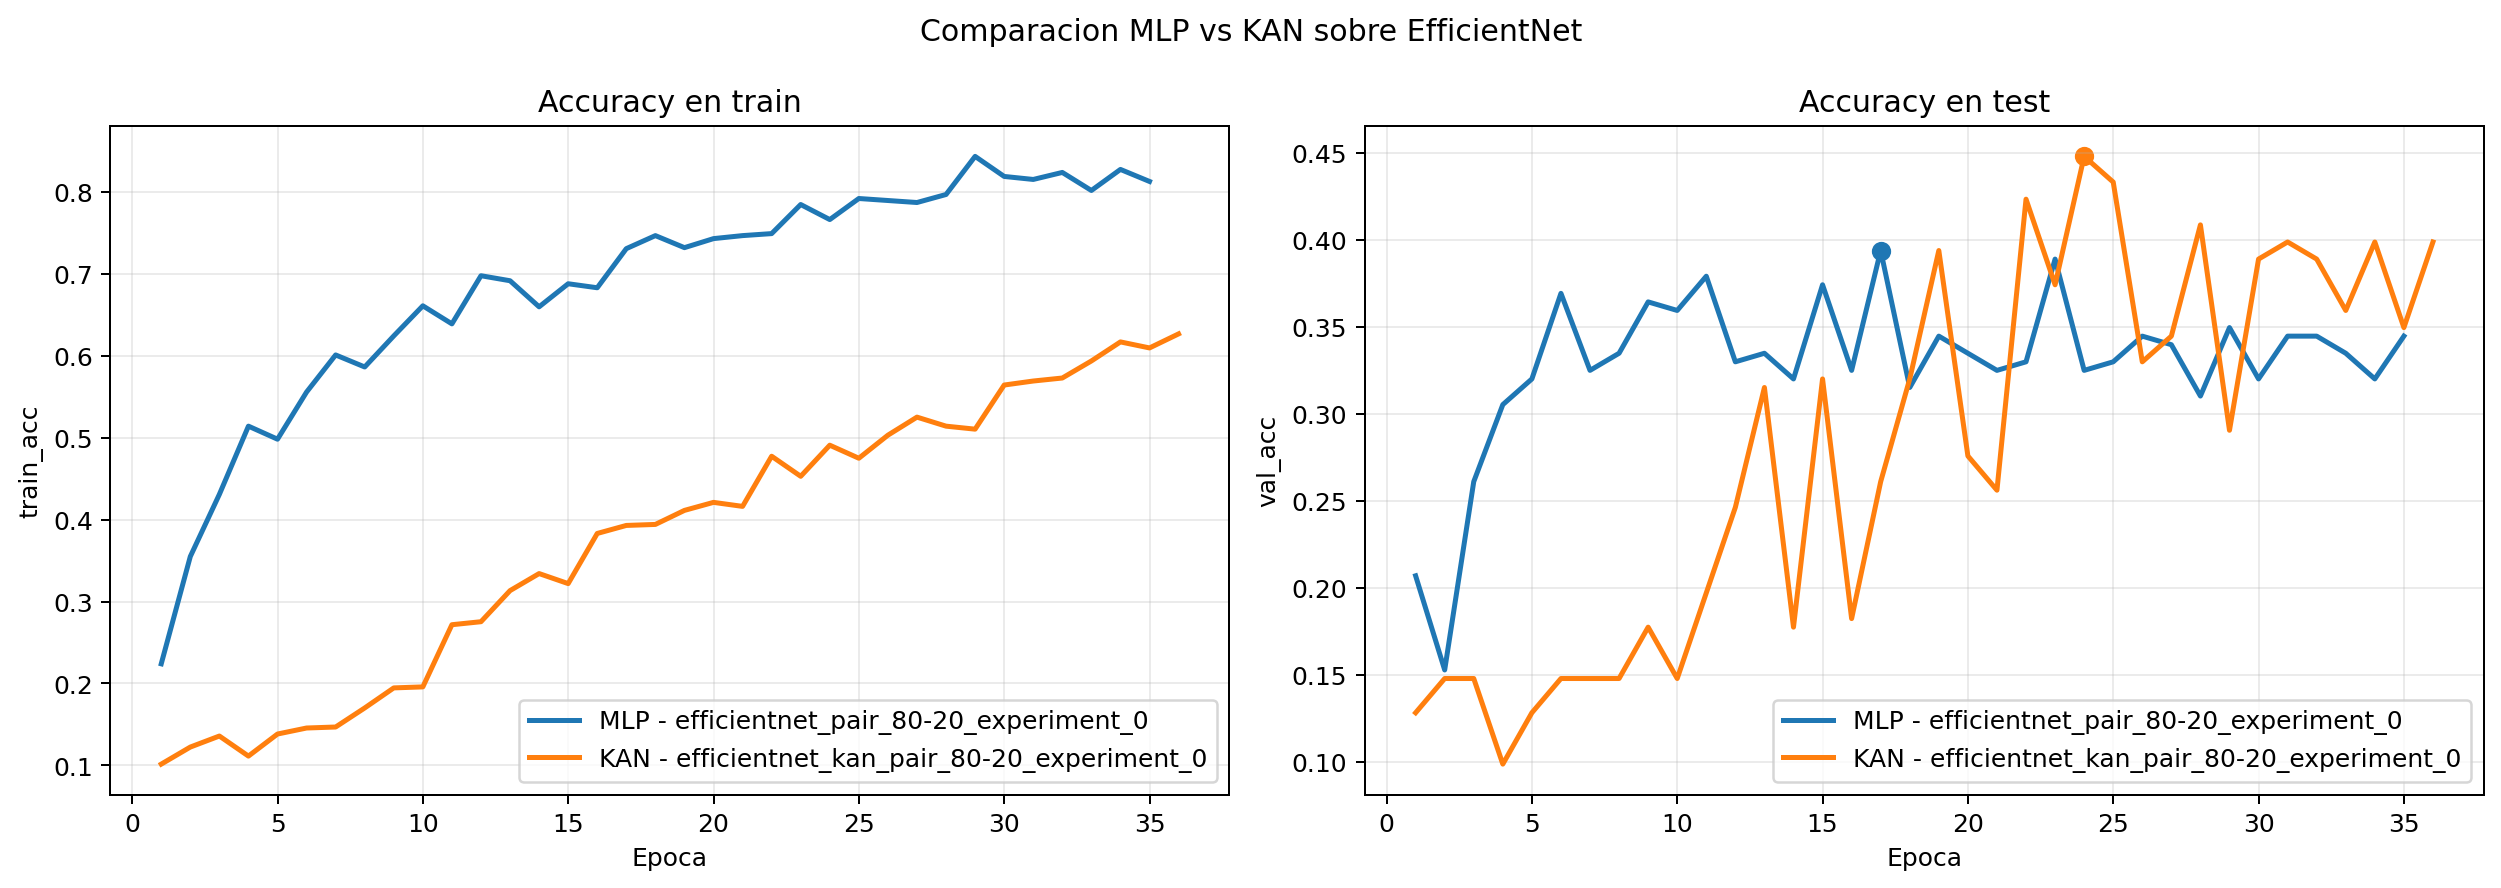
\includegraphics[width=\linewidth]{efficientnet_comparacion_mlp_kan.png}
\end{columns}
\end{frame}

\begin{frame}{Bloque 2: curva con m\'etrica h\'ibrida}
\centering
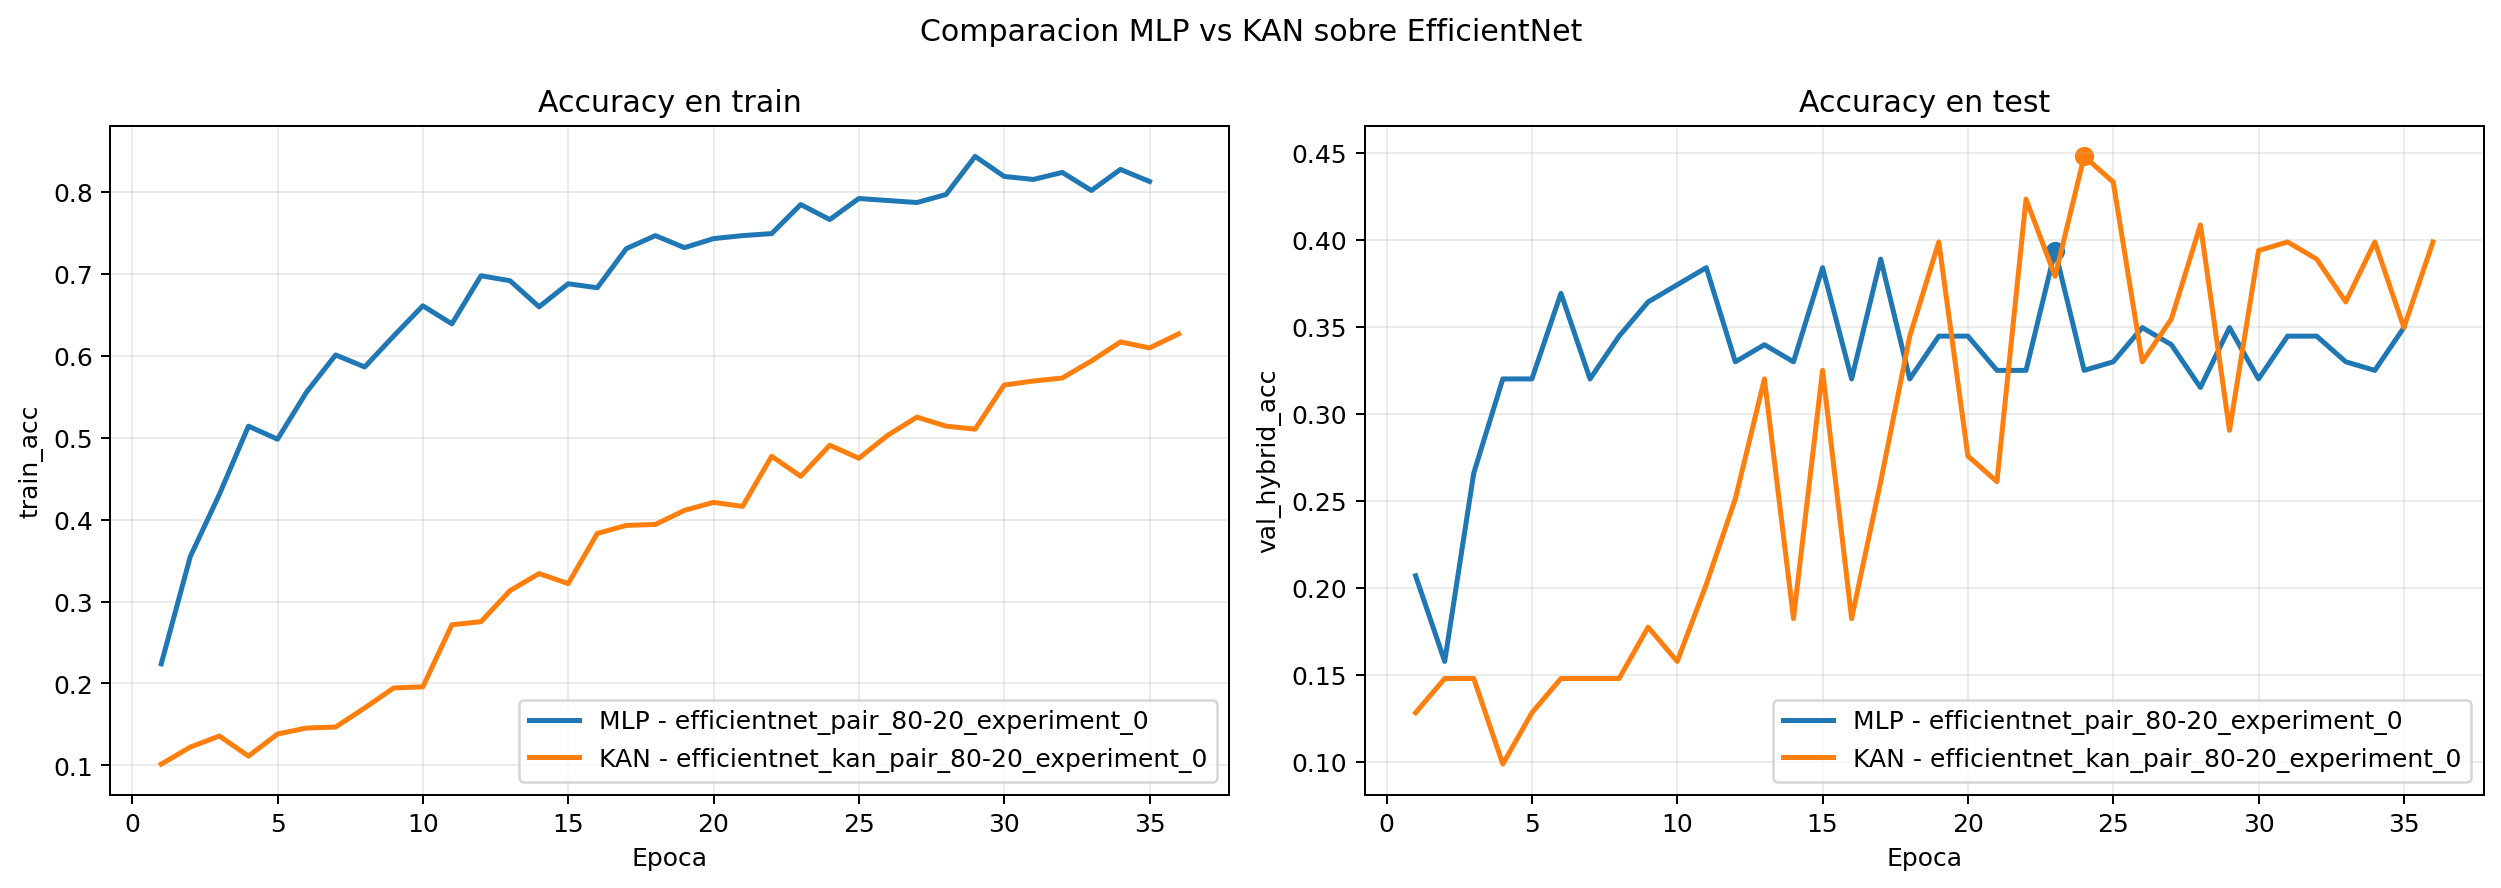
\includegraphics[width=0.88\textwidth]{efficientnet_comparacion_mlp_kan_hybrid.png}
\end{frame}

\begin{frame}{Bloque 2: ejemplos visuales de EfficientNet + MLP}
\centering
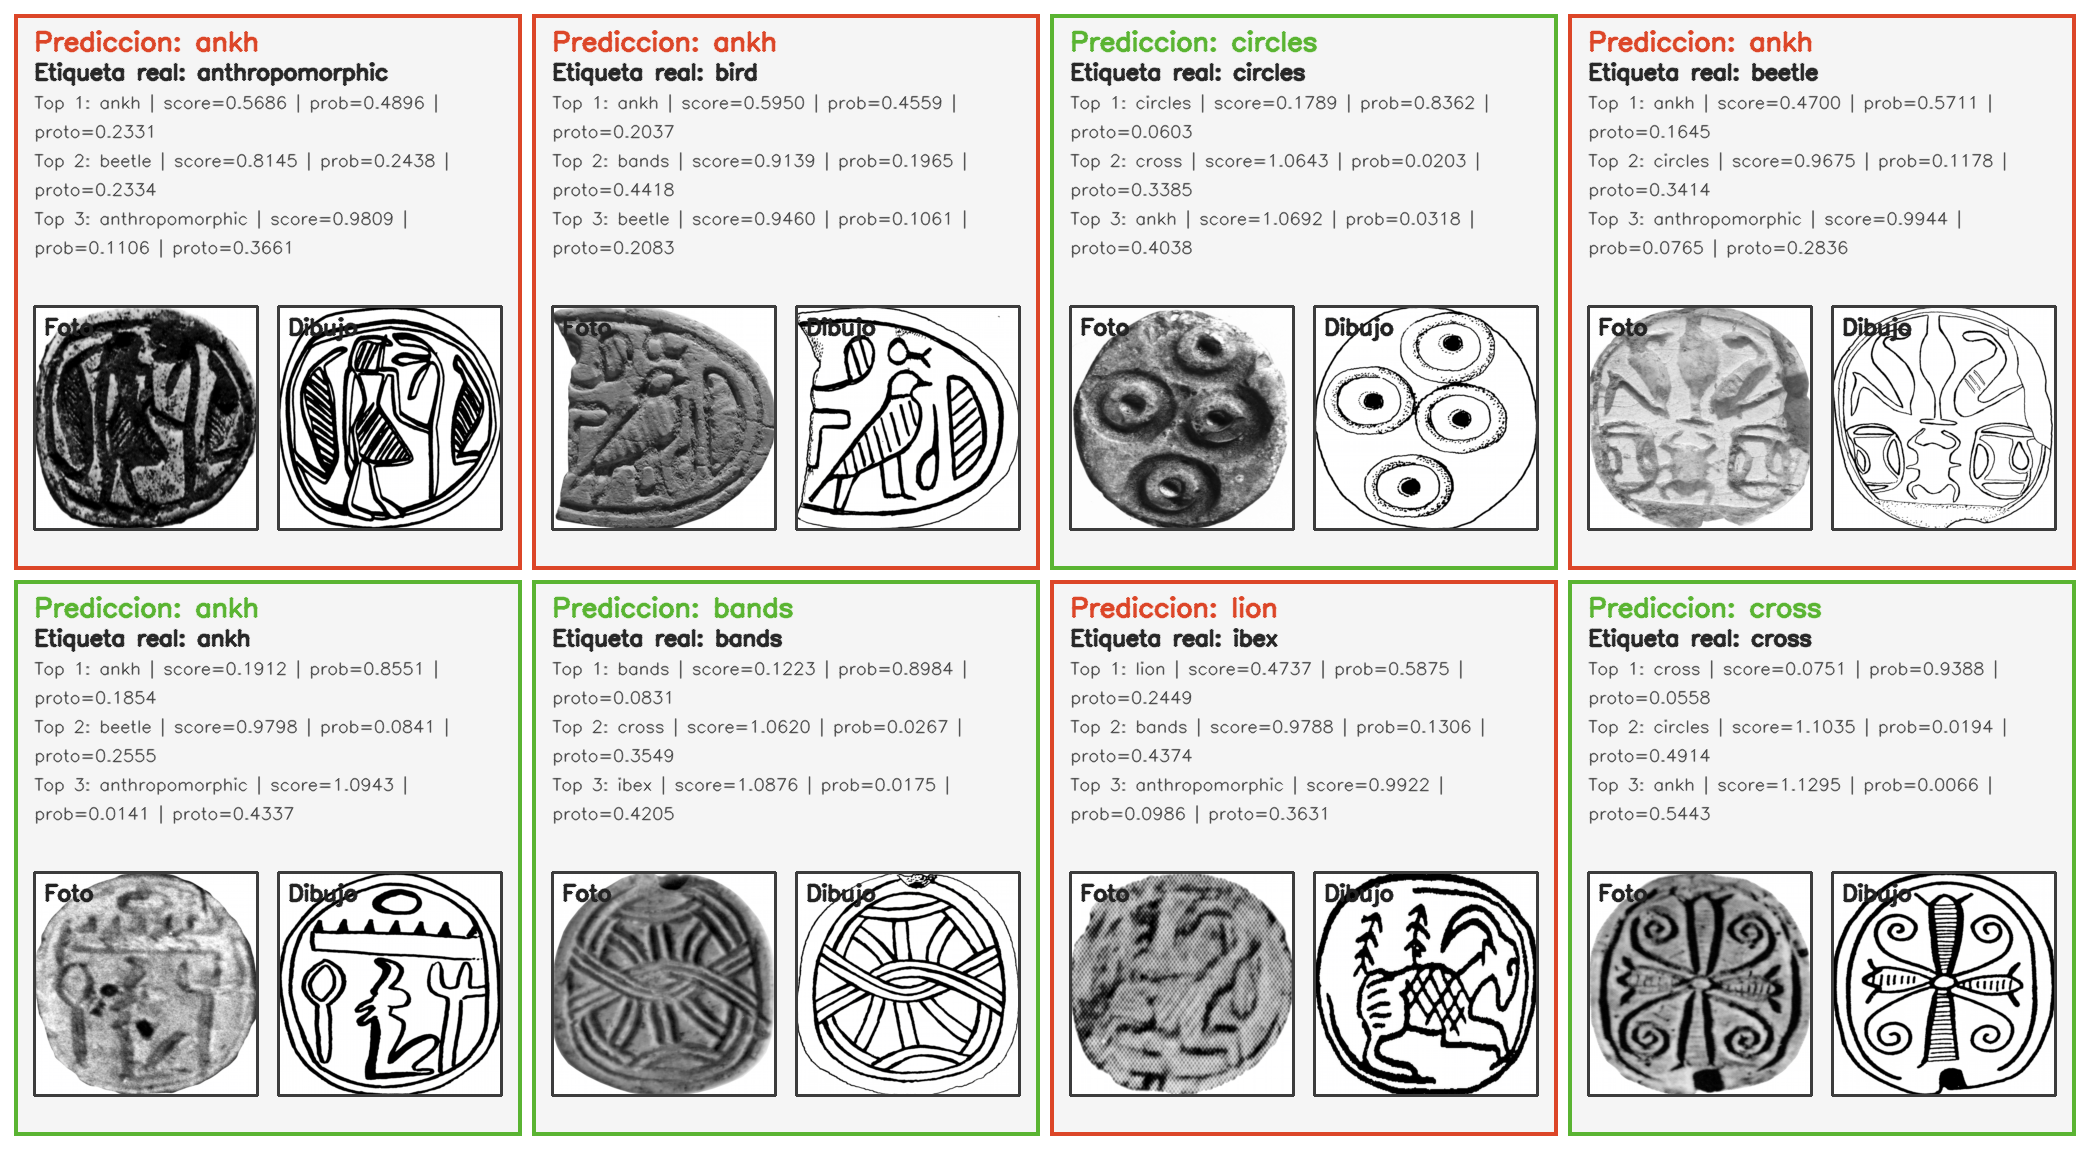
\includegraphics[width=\textwidth]{efficientnet_mlp_mosaico_horizontal.png}
\end{frame}

\begin{frame}{Bloque 2: ejemplos visuales de EfficientNet + KAN}
\centering
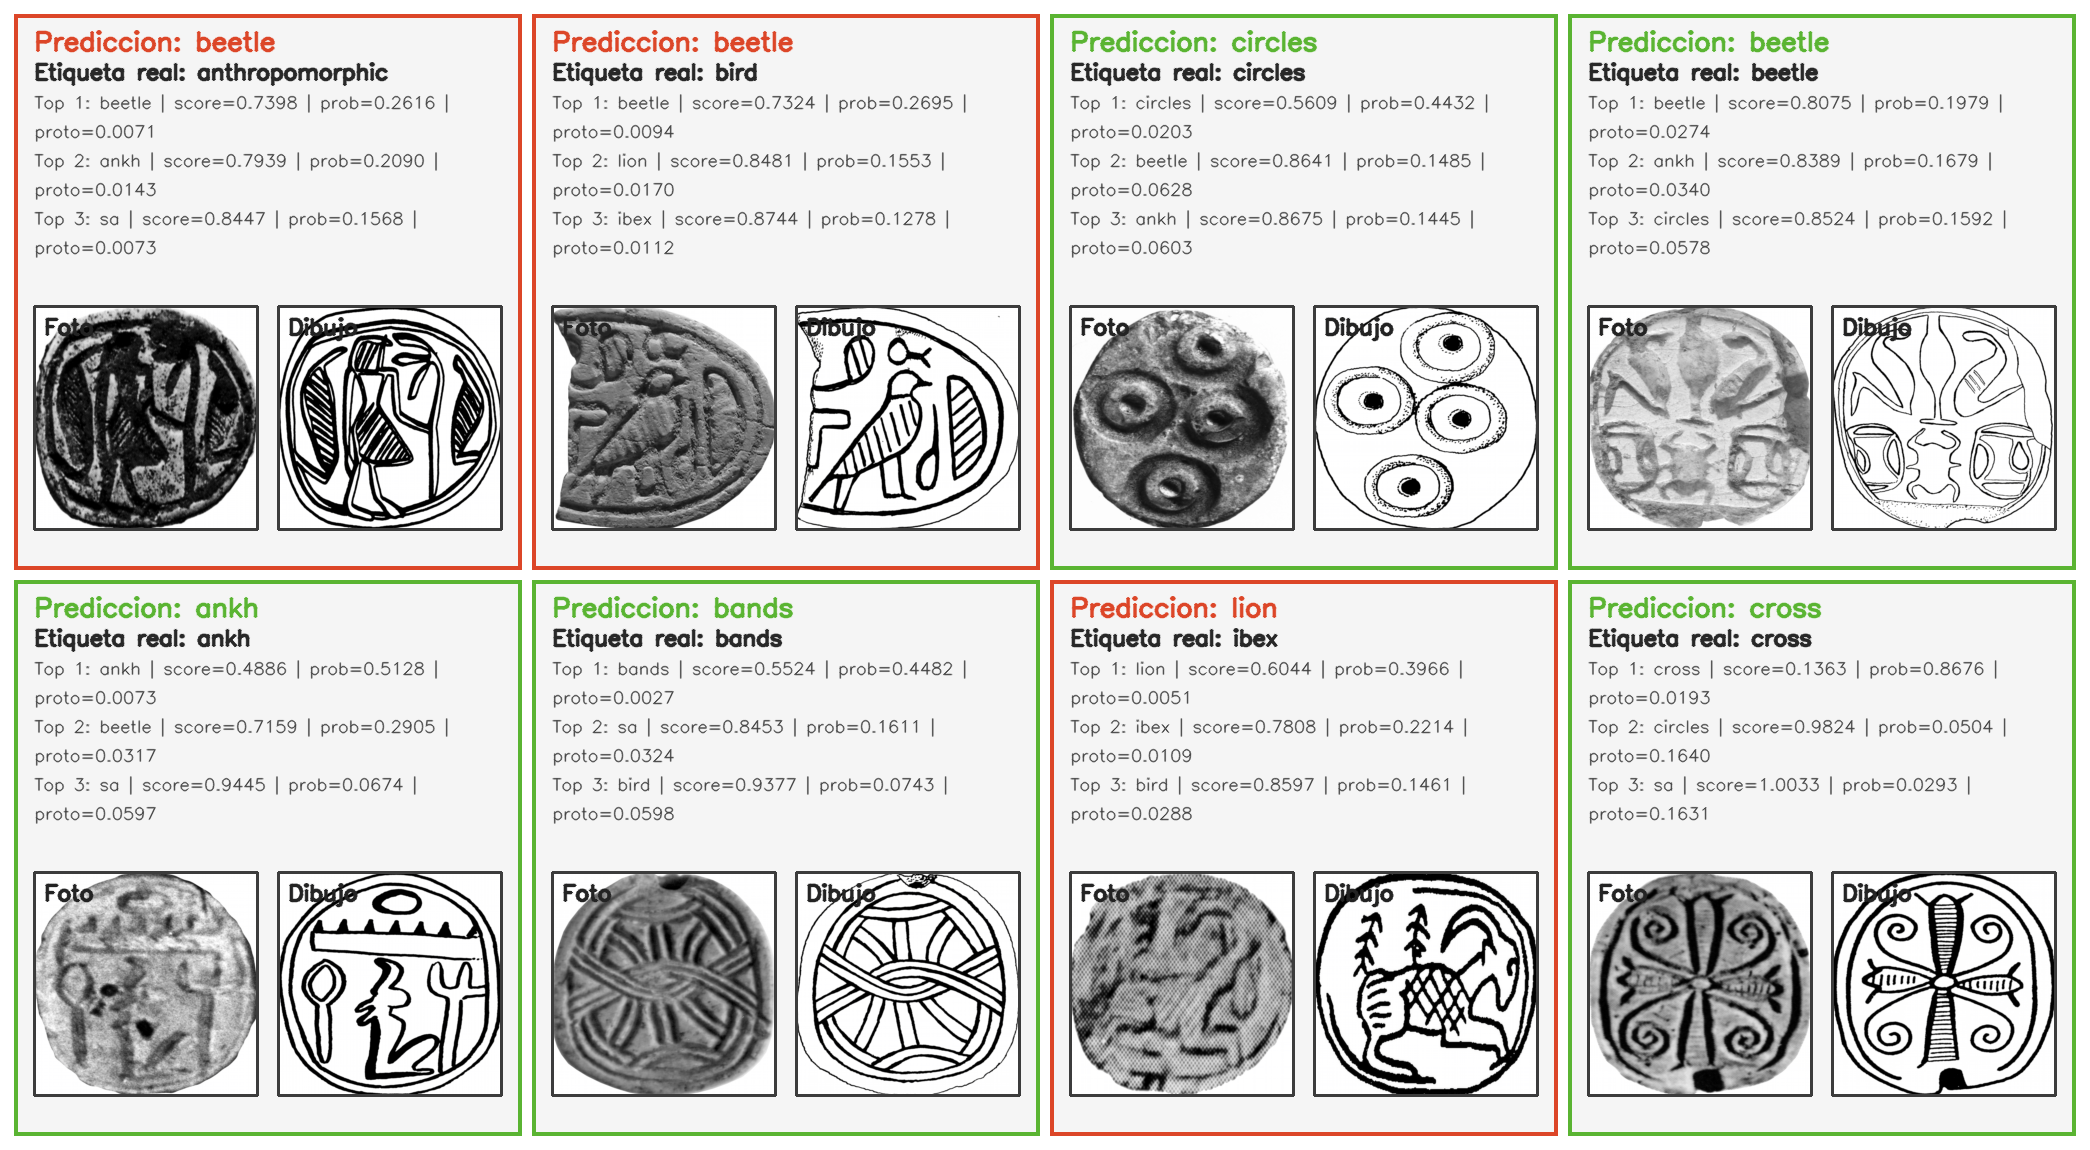
\includegraphics[width=\textwidth]{efficientnet_kan_mosaico_horizontal.png}
\end{frame}

\begin{frame}{Mensaje final}
\Large
\begin{itemize}
  \item En modelos ligeros, KAN no mejora de forma clara a MLP.
  \item Con \texttt{EfficientNet-B0}, la cabeza KAN s\'i ofrece una mejora visible.
  \item La utilidad de KAN depende de la calidad de la representaci\'on de entrada.
\end{itemize}

\vspace{0.5cm}
\centering
\Large{Gracias por vuestra atenci\'on}
\end{frame}

\end{document}
